\documentclass[1p]{elsarticle_modified}
%\bibliographystyle{elsarticle-num}

%\usepackage[colorlinks]{hyperref}
%\usepackage{abbrmath_seonhwa} %\Abb, \Ascr, \Acal ,\Abf, \Afrak
\usepackage{amsfonts}
\usepackage{amssymb}
\usepackage{amsmath}
\usepackage{amsthm}
\usepackage{scalefnt}
\usepackage{amsbsy}
\usepackage{kotex}
\usepackage{caption}
\usepackage{subfig}
\usepackage{color}
\usepackage{graphicx}
\usepackage{xcolor} %% white, black, red, green, blue, cyan, magenta, yellow
\usepackage{float}
\usepackage{setspace}
\usepackage{hyperref}

\usepackage{tikz}
\usetikzlibrary{arrows}

\usepackage{multirow}
\usepackage{array} % fixed length table
\usepackage{hhline}

%%%%%%%%%%%%%%%%%%%%%
\makeatletter
\renewcommand*\env@matrix[1][\arraystretch]{%
	\edef\arraystretch{#1}%
	\hskip -\arraycolsep
	\let\@ifnextchar\new@ifnextchar
	\array{*\c@MaxMatrixCols c}}
\makeatother %https://tex.stackexchange.com/questions/14071/how-can-i-increase-the-line-spacing-in-a-matrix
%%%%%%%%%%%%%%%

\usepackage[normalem]{ulem}

\newcommand{\msout}[1]{\ifmmode\text{\sout{\ensuremath{#1}}}\else\sout{#1}\fi}
%SOURCE: \msout is \stkout macro in https://tex.stackexchange.com/questions/20609/strikeout-in-math-mode

\newcommand{\cancel}[1]{
	\ifmmode
	{\color{red}\msout{#1}}
	\else
	{\color{red}\sout{#1}}
	\fi
}

\newcommand{\add}[1]{
	{\color{blue}\uwave{#1}}
}

\newcommand{\replace}[2]{
	\ifmmode
	{\color{red}\msout{#1}}{\color{blue}\uwave{#2}}
	\else
	{\color{red}\sout{#1}}{\color{blue}\uwave{#2}}
	\fi
}

\newcommand{\Sol}{\mathcal{S}} %segment
\newcommand{\D}{D} %diagram
\newcommand{\A}{\mathcal{A}} %arc


%%%%%%%%%%%%%%%%%%%%%%%%%%%%%5 test

\def\sl{\operatorname{\textup{SL}}(2,\Cbb)}
\def\psl{\operatorname{\textup{PSL}}(2,\Cbb)}
\def\quan{\mkern 1mu \triangleright \mkern 1mu}

\theoremstyle{definition}
\newtheorem{thm}{Theorem}[section]
\newtheorem{prop}[thm]{Proposition}
\newtheorem{lem}[thm]{Lemma}
\newtheorem{ques}[thm]{Question}
\newtheorem{cor}[thm]{Corollary}
\newtheorem{defn}[thm]{Definition}
\newtheorem{exam}[thm]{Example}
\newtheorem{rmk}[thm]{Remark}
\newtheorem{alg}[thm]{Algorithm}

\newcommand{\I}{\sqrt{-1}}
\begin{document}

%\begin{frontmatter}
%
%\title{Boundary parabolic representations of knots up to 8 crossings}
%
%%% Group authors per affiliation:
%\author{Yunhi Cho} 
%\address{Department of Mathematics, University of Seoul, Seoul, Korea}
%\ead{yhcho@uos.ac.kr}
%
%
%\author{Seonhwa Kim} %\fnref{s_kim}}
%\address{Center for Geometry and Physics, Institute for Basic Science, Pohang, 37673, Korea}
%\ead{ryeona17@ibs.re.kr}
%
%\author{Hyuk Kim}
%\address{Department of Mathematical Sciences, Seoul National University, Seoul 08826, Korea}
%\ead{hyukkim@snu.ac.kr}
%
%\author{Seokbeom Yoon}
%\address{Department of Mathematical Sciences, Seoul National University, Seoul, 08826,  Korea}
%\ead{sbyoon15@snu.ac.kr}
%
%\begin{abstract}
%We find all boundary parabolic representation of knots up to 8 crossings.
%
%\end{abstract}
%\begin{keyword}
%    \MSC[2010] 57M25 
%\end{keyword}
%
%\end{frontmatter}

%\linenumbers
%\tableofcontents
%
\newcommand\colored[1]{\textcolor{white}{\rule[-0.35ex]{0.8em}{1.4ex}}\kern-0.8em\color{red} #1}%
%\newcommand\colored[1]{\textcolor{white}{ #1}\kern-2.17ex	\textcolor{white}{ #1}\kern-1.81ex	\textcolor{white}{ #1}\kern-2.15ex\color{red}#1	}

{\Large $\underline{12a_{1258}~(K12a_{1258})}$}

\setlength{\tabcolsep}{10pt}
\renewcommand{\arraystretch}{1.6}
\vspace{1cm}\begin{tabular}{m{100pt}>{\centering\arraybackslash}m{274pt}}
\multirow{5}{120pt}{
	\centering
	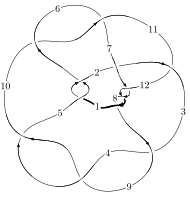
\includegraphics[width=112pt]{../../../GIT/diagram.site/Diagrams/png/2059_12a_1258.png}\\
\ \ \ A knot diagram\footnotemark}&
\allowdisplaybreaks
\textbf{Linearized knot diagam} \\
\cline{2-2}
 &
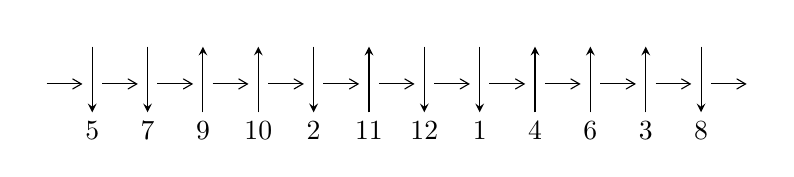
\begin{tikzpicture}[x=20pt, y=17pt]
	% nodes
	\node (C0) at (0, 0) {};
	\node (C1) at (1, 0) {};
	\node (C1U) at (1, +1) {};
	\node (C1D) at (1, -1) {5};

	\node (C2) at (2, 0) {};
	\node (C2U) at (2, +1) {};
	\node (C2D) at (2, -1) {7};

	\node (C3) at (3, 0) {};
	\node (C3U) at (3, +1) {};
	\node (C3D) at (3, -1) {9};

	\node (C4) at (4, 0) {};
	\node (C4U) at (4, +1) {};
	\node (C4D) at (4, -1) {10};

	\node (C5) at (5, 0) {};
	\node (C5U) at (5, +1) {};
	\node (C5D) at (5, -1) {2};

	\node (C6) at (6, 0) {};
	\node (C6U) at (6, +1) {};
	\node (C6D) at (6, -1) {11};

	\node (C7) at (7, 0) {};
	\node (C7U) at (7, +1) {};
	\node (C7D) at (7, -1) {12};

	\node (C8) at (8, 0) {};
	\node (C8U) at (8, +1) {};
	\node (C8D) at (8, -1) {1};

	\node (C9) at (9, 0) {};
	\node (C9U) at (9, +1) {};
	\node (C9D) at (9, -1) {4};

	\node (C10) at (10, 0) {};
	\node (C10U) at (10, +1) {};
	\node (C10D) at (10, -1) {6};

	\node (C11) at (11, 0) {};
	\node (C11U) at (11, +1) {};
	\node (C11D) at (11, -1) {3};

	\node (C12) at (12, 0) {};
	\node (C12U) at (12, +1) {};
	\node (C12D) at (12, -1) {8};
	\node (C13) at (13, 0) {};

	% arrows
	\draw[->,>={angle 60}]
	(C0) edge (C1) (C1) edge (C2) (C2) edge (C3) (C3) edge (C4) (C4) edge (C5) (C5) edge (C6) (C6) edge (C7) (C7) edge (C8) (C8) edge (C9) (C9) edge (C10) (C10) edge (C11) (C11) edge (C12) (C12) edge (C13) ;	\draw[->,>=stealth]
	(C1U) edge (C1D) (C2U) edge (C2D) (C3D) edge (C3U) (C4D) edge (C4U) (C5U) edge (C5D) (C6D) edge (C6U) (C7U) edge (C7D) (C8U) edge (C8D) (C9D) edge (C9U) (C10D) edge (C10U) (C11D) edge (C11U) (C12U) edge (C12D) ;
	\end{tikzpicture} \\
\hhline{~~} \\& 
\textbf{Solving Sequence} \\ \cline{2-2} 
 &
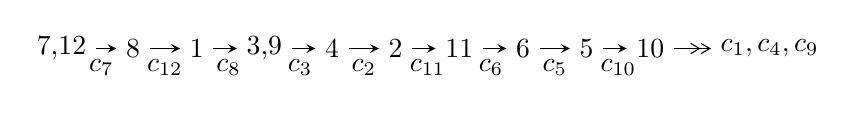
\begin{tikzpicture}[x=23pt, y=7pt]
	% node
	\node (A0) at (-1/8, 0) {7,12};
	\node (A1) at (1, 0) {8};
	\node (A2) at (2, 0) {1};
	\node (A3) at (49/16, 0) {3,9};
	\node (A4) at (33/8, 0) {4};
	\node (A5) at (41/8, 0) {2};
	\node (A6) at (49/8, 0) {11};
	\node (A7) at (57/8, 0) {6};
	\node (A8) at (65/8, 0) {5};
	\node (A9) at (73/8, 0) {10};
	\node (C1) at (1/2, -1) {$c_{7}$};
	\node (C2) at (3/2, -1) {$c_{12}$};
	\node (C3) at (5/2, -1) {$c_{8}$};
	\node (C4) at (29/8, -1) {$c_{3}$};
	\node (C5) at (37/8, -1) {$c_{2}$};
	\node (C6) at (45/8, -1) {$c_{11}$};
	\node (C7) at (53/8, -1) {$c_{6}$};
	\node (C8) at (61/8, -1) {$c_{5}$};
	\node (C9) at (69/8, -1) {$c_{10}$};
	\node (A10) at (11, 0) {$c_{1},c_{4},c_{9}$};

	% edge
	\draw[->,>=stealth]	
	(A0) edge (A1) (A1) edge (A2) (A2) edge (A3) (A3) edge (A4) (A4) edge (A5) (A5) edge (A6) (A6) edge (A7) (A7) edge (A8) (A8) edge (A9) ;
	\draw[->>,>={angle 60}]	
	(A9) edge (A10);
\end{tikzpicture} \\ 

\end{tabular} \\

\footnotetext{
The image of knot diagram is generated by the software ``\textbf{Draw programme}" developed by Andrew Bartholomew(\url{http://www.layer8.co.uk/maths/draw/index.htm\#Running-draw}), where we modified some parts for our purpose(\url{https://github.com/CATsTAILs/LinksPainter}).
}\phantom \\ \newline 
\centering \textbf{Ideals for irreducible components\footnotemark of $X_{\text{par}}$} 
 
\begin{align*}
I^u_{1}&=\langle 
-2.55261\times10^{241} u^{98}-6.00163\times10^{241} u^{97}+\cdots+4.24303\times10^{242} b-1.66484\times10^{242},\\
\phantom{I^u_{1}}&\phantom{= \langle  }-4.48746\times10^{242} u^{98}-1.03495\times10^{243} u^{97}+\cdots+2.30336\times10^{243} a-1.49280\times10^{244},\\
\phantom{I^u_{1}}&\phantom{= \langle  }u^{99}+3 u^{98}+\cdots+74 u+19\rangle \\
I^u_{2}&=\langle 
u^{20}+u^{19}+\cdots+b+1,\;11 u^{20}+6 u^{19}+\cdots+2 a+23,\;u^{21}-14 u^{19}+\cdots+u-1\rangle \\
\\
\end{align*}
\raggedright * 2 irreducible components of $\dim_{\mathbb{C}}=0$, with total 120 representations.\\
\footnotetext{All coefficients of polynomials are rational numbers. But the coefficients are sometimes approximated in decimal forms when there is not enough margin.}
\newpage
\renewcommand{\arraystretch}{1}
\centering \section*{I. $I^u_{1}= \langle -2.55\times10^{241} u^{98}-6.00\times10^{241} u^{97}+\cdots+4.24\times10^{242} b-1.66\times10^{242},\;-4.49\times10^{242} u^{98}-1.03\times10^{243} u^{97}+\cdots+2.30\times10^{243} a-1.49\times10^{244},\;u^{99}+3 u^{98}+\cdots+74 u+19 \rangle$}
\flushleft \textbf{(i) Arc colorings}\\
\begin{tabular}{m{7pt} m{180pt} m{7pt} m{180pt} }
\flushright $a_{7}=$&$\begin{pmatrix}1\\0\end{pmatrix}$ \\
\flushright $a_{12}=$&$\begin{pmatrix}0\\u\end{pmatrix}$ \\
\flushright $a_{8}=$&$\begin{pmatrix}1\\u^2\end{pmatrix}$ \\
\flushright $a_{1}=$&$\begin{pmatrix}- u\\- u^3+u\end{pmatrix}$ \\
\flushright $a_{3}=$&$\begin{pmatrix}0.194822 u^{98}+0.449324 u^{97}+\cdots+23.8610 u+6.48099\\0.0601601 u^{98}+0.141447 u^{97}+\cdots+1.99506 u+0.392369\end{pmatrix}$ \\
\flushright $a_{9}=$&$\begin{pmatrix}- u^2+1\\- u^4+2 u^2\end{pmatrix}$ \\
\flushright $a_{4}=$&$\begin{pmatrix}0.292740 u^{98}+0.655874 u^{97}+\cdots+30.4673 u+7.32334\\0.0214966 u^{98}+0.0592174 u^{97}+\cdots+0.553157 u+0.0275512\end{pmatrix}$ \\
\flushright $a_{2}=$&$\begin{pmatrix}0.254983 u^{98}+0.590771 u^{97}+\cdots+25.8561 u+6.87336\\0.0601601 u^{98}+0.141447 u^{97}+\cdots+1.99506 u+0.392369\end{pmatrix}$ \\
\flushright $a_{11}=$&$\begin{pmatrix}0.0406568 u^{98}+0.0789464 u^{97}+\cdots+5.22744 u-0.333209\\0.0270023 u^{98}+0.0262813 u^{97}+\cdots+1.59997 u+0.408942\end{pmatrix}$ \\
\flushright $a_{6}=$&$\begin{pmatrix}0.123531 u^{98}+0.319533 u^{97}+\cdots+12.3956 u+5.03543\\0.100580 u^{98}+0.217161 u^{97}+\cdots+7.38599 u+1.96953\end{pmatrix}$ \\
\flushright $a_{5}=$&$\begin{pmatrix}0.141766 u^{98}+0.350890 u^{97}+\cdots+17.4096 u+3.36732\\0.0519563 u^{98}+0.120722 u^{97}+\cdots+3.19261 u+0.366127\end{pmatrix}$ \\
\flushright $a_{10}=$&$\begin{pmatrix}0.0473159 u^{98}+0.197736 u^{97}+\cdots+21.0124 u-0.138025\\-0.0392609 u^{98}-0.00751575 u^{97}+\cdots-3.64472 u-1.70638\end{pmatrix}$\\&\end{tabular}
\flushleft \textbf{(ii) Obstruction class $= -1$}\\~\\
\flushleft \textbf{(iii) Cusp Shapes $= -0.432175 u^{98}-1.12277 u^{97}+\cdots-14.7712 u-6.70211$}\\~\\
\newpage\renewcommand{\arraystretch}{1}
\flushleft \textbf{(iv) u-Polynomials at the component}\newline \\
\begin{tabular}{m{50pt}|m{274pt}}
Crossings & \hspace{64pt}u-Polynomials at each crossing \\
\hline $$\begin{aligned}c_{1},c_{5}\end{aligned}$$&$\begin{aligned}
&u^{99}-2 u^{98}+\cdots-168 u+49
\end{aligned}$\\
\hline $$\begin{aligned}c_{2}\end{aligned}$$&$\begin{aligned}
&u^{99}-2 u^{98}+\cdots+163 u+17
\end{aligned}$\\
\hline $$\begin{aligned}c_{3},c_{4},c_{9}\end{aligned}$$&$\begin{aligned}
&u^{99}- u^{98}+\cdots-634 u-23
\end{aligned}$\\
\hline $$\begin{aligned}c_{6},c_{10}\end{aligned}$$&$\begin{aligned}
&u^{99}-36 u^{97}+\cdots+52 u-7
\end{aligned}$\\
\hline $$\begin{aligned}c_{7},c_{8},c_{12}\end{aligned}$$&$\begin{aligned}
&u^{99}-3 u^{98}+\cdots+74 u-19
\end{aligned}$\\
\hline $$\begin{aligned}c_{11}\end{aligned}$$&$\begin{aligned}
&u^{99}-5 u^{98}+\cdots+465 u^2-1
\end{aligned}$\\
\hline
\end{tabular}\\~\\
\newpage\renewcommand{\arraystretch}{1}
\flushleft \textbf{(v) Riley Polynomials at the component}\newline \\
\begin{tabular}{m{50pt}|m{274pt}}
Crossings & \hspace{64pt}Riley Polynomials at each crossing \\
\hline $$\begin{aligned}c_{1},c_{5}\end{aligned}$$&$\begin{aligned}
&y^{99}-60 y^{98}+\cdots+121030 y-2401
\end{aligned}$\\
\hline $$\begin{aligned}c_{2}\end{aligned}$$&$\begin{aligned}
&y^{99}-20 y^{98}+\cdots+25889 y-289
\end{aligned}$\\
\hline $$\begin{aligned}c_{3},c_{4},c_{9}\end{aligned}$$&$\begin{aligned}
&y^{99}-95 y^{98}+\cdots+306322 y-529
\end{aligned}$\\
\hline $$\begin{aligned}c_{6},c_{10}\end{aligned}$$&$\begin{aligned}
&y^{99}-72 y^{98}+\cdots+660 y-49
\end{aligned}$\\
\hline $$\begin{aligned}c_{7},c_{8},c_{12}\end{aligned}$$&$\begin{aligned}
&y^{99}-103 y^{98}+\cdots-6038 y-361
\end{aligned}$\\
\hline $$\begin{aligned}c_{11}\end{aligned}$$&$\begin{aligned}
&y^{99}-7 y^{98}+\cdots+930 y-1
\end{aligned}$\\
\hline
\end{tabular}\\~\\
\newpage\flushleft \textbf{(vi) Complex Volumes and Cusp Shapes}
$$\begin{array}{c|c|c}  
\text{Solutions to }I^u_{1}& \I (\text{vol} + \sqrt{-1}CS) & \text{Cusp shape}\\
 \hline 
\begin{aligned}
u &= \phantom{-}0.638994 + 0.739104 I \\
a &= \phantom{-}0.228661 + 0.744090 I \\
b &= -0.793896 - 0.324299 I\end{aligned}
 & -3.35882 - 2.76331 I & \phantom{-0.000000 } 0 \\ \hline\begin{aligned}
u &= \phantom{-}0.638994 - 0.739104 I \\
a &= \phantom{-}0.228661 - 0.744090 I \\
b &= -0.793896 + 0.324299 I\end{aligned}
 & -3.35882 + 2.76331 I & \phantom{-0.000000 } 0 \\ \hline\begin{aligned}
u &= \phantom{-}0.511185 + 0.944135 I \\
a &= \phantom{-}0.163975 + 1.264040 I \\
b &= -1.00260 - 1.02085 I\end{aligned}
 & \phantom{-}6.54384 - 12.43480 I & \phantom{-0.000000 } 0 \\ \hline\begin{aligned}
u &= \phantom{-}0.511185 - 0.944135 I \\
a &= \phantom{-}0.163975 - 1.264040 I \\
b &= -1.00260 + 1.02085 I\end{aligned}
 & \phantom{-}6.54384 + 12.43480 I & \phantom{-0.000000 } 0 \\ \hline\begin{aligned}
u &= \phantom{-}0.540446 + 0.735322 I \\
a &= \phantom{-}0.18350 - 1.66701 I \\
b &= \phantom{-}0.911733 + 0.865941 I\end{aligned}
 & \phantom{-}9.94163 - 5.42512 I & \phantom{-0.000000 } 0 \\ \hline\begin{aligned}
u &= \phantom{-}0.540446 - 0.735322 I \\
a &= \phantom{-}0.18350 + 1.66701 I \\
b &= \phantom{-}0.911733 - 0.865941 I\end{aligned}
 & \phantom{-}9.94163 + 5.42512 I & \phantom{-0.000000 } 0 \\ \hline\begin{aligned}
u &= -0.172232 + 0.883812 I \\
a &= \phantom{-}0.754439 - 0.973326 I \\
b &= -0.587200 + 0.722324 I\end{aligned}
 & \phantom{-}3.85491 + 2.48956 I & \phantom{-0.000000 } 0 \\ \hline\begin{aligned}
u &= -0.172232 - 0.883812 I \\
a &= \phantom{-}0.754439 + 0.973326 I \\
b &= -0.587200 - 0.722324 I\end{aligned}
 & \phantom{-}3.85491 - 2.48956 I & \phantom{-0.000000 } 0 \\ \hline\begin{aligned}
u &= -0.879167 + 0.061143 I \\
a &= \phantom{-}1.384480 + 0.052534 I \\
b &= \phantom{-}0.184132 - 0.062040 I\end{aligned}
 & \phantom{-}2.42479 - 0.00213 I & \phantom{-0.000000 } 0 \\ \hline\begin{aligned}
u &= -0.879167 - 0.061143 I \\
a &= \phantom{-}1.384480 - 0.052534 I \\
b &= \phantom{-}0.184132 + 0.062040 I\end{aligned}
 & \phantom{-}2.42479 + 0.00213 I & \phantom{-0.000000 } 0\\
 \hline 
 \end{array}$$\newpage$$\begin{array}{c|c|c}  
\text{Solutions to }I^u_{1}& \I (\text{vol} + \sqrt{-1}CS) & \text{Cusp shape}\\
 \hline 
\begin{aligned}
u &= -0.415960 + 0.773865 I \\
a &= -0.952838 - 0.274165 I \\
b &= \phantom{-}0.563722 + 0.793689 I\end{aligned}
 & \phantom{-}0.74742 - 3.86475 I & \phantom{-0.000000 } 0 \\ \hline\begin{aligned}
u &= -0.415960 - 0.773865 I \\
a &= -0.952838 + 0.274165 I \\
b &= \phantom{-}0.563722 - 0.793689 I\end{aligned}
 & \phantom{-}0.74742 + 3.86475 I & \phantom{-0.000000 } 0 \\ \hline\begin{aligned}
u &= \phantom{-}1.062410 + 0.380284 I \\
a &= -1.144630 + 0.599349 I \\
b &= -1.39357 - 0.51108 I\end{aligned}
 & \phantom{-}3.54258 + 0.66396 I & \phantom{-0.000000 } 0 \\ \hline\begin{aligned}
u &= \phantom{-}1.062410 - 0.380284 I \\
a &= -1.144630 - 0.599349 I \\
b &= -1.39357 + 0.51108 I\end{aligned}
 & \phantom{-}3.54258 - 0.66396 I & \phantom{-0.000000 } 0 \\ \hline\begin{aligned}
u &= -0.513689 + 0.678395 I \\
a &= -0.10183 + 1.44799 I \\
b &= \phantom{-}1.03582 - 1.05461 I\end{aligned}
 & \phantom{-}0.41702 + 8.50479 I & \phantom{-0.000000 } 0 \\ \hline\begin{aligned}
u &= -0.513689 - 0.678395 I \\
a &= -0.10183 - 1.44799 I \\
b &= \phantom{-}1.03582 + 1.05461 I\end{aligned}
 & \phantom{-}0.41702 - 8.50479 I & \phantom{-0.000000 } 0 \\ \hline\begin{aligned}
u &= -0.425029 + 1.086770 I \\
a &= -0.413391 + 0.592418 I \\
b &= \phantom{-}0.700812 - 0.301259 I\end{aligned}
 & \phantom{-}1.91325 + 5.57658 I & \phantom{-0.000000 } 0 \\ \hline\begin{aligned}
u &= -0.425029 - 1.086770 I \\
a &= -0.413391 - 0.592418 I \\
b &= \phantom{-}0.700812 + 0.301259 I\end{aligned}
 & \phantom{-}1.91325 - 5.57658 I & \phantom{-0.000000 } 0 \\ \hline\begin{aligned}
u &= \phantom{-}0.496443 + 0.664464 I \\
a &= -0.910416 + 0.679661 I \\
b &= \phantom{-}0.816921 - 0.775446 I\end{aligned}
 & \phantom{-}9.99441 + 0.67991 I & \phantom{-0.000000 } 0 \\ \hline\begin{aligned}
u &= \phantom{-}0.496443 - 0.664464 I \\
a &= -0.910416 - 0.679661 I \\
b &= \phantom{-}0.816921 + 0.775446 I\end{aligned}
 & \phantom{-}9.99441 - 0.67991 I & \phantom{-0.000000 } 0\\
 \hline 
 \end{array}$$\newpage$$\begin{array}{c|c|c}  
\text{Solutions to }I^u_{1}& \I (\text{vol} + \sqrt{-1}CS) & \text{Cusp shape}\\
 \hline 
\begin{aligned}
u &= \phantom{-}0.743531 + 0.998930 I \\
a &= \phantom{-}0.594722 - 0.257668 I \\
b &= -0.597670 + 0.831620 I\end{aligned}
 & \phantom{-}5.97682 + 6.13788 I & \phantom{-0.000000 } 0 \\ \hline\begin{aligned}
u &= \phantom{-}0.743531 - 0.998930 I \\
a &= \phantom{-}0.594722 + 0.257668 I \\
b &= -0.597670 - 0.831620 I\end{aligned}
 & \phantom{-}5.97682 - 6.13788 I & \phantom{-0.000000 } 0 \\ \hline\begin{aligned}
u &= \phantom{-}1.251660 + 0.031833 I \\
a &= -0.0696663 + 0.0094888 I \\
b &= -0.49160 - 1.82486 I\end{aligned}
 & -1.66463 - 2.28211 I & \phantom{-0.000000 } 0 \\ \hline\begin{aligned}
u &= \phantom{-}1.251660 - 0.031833 I \\
a &= -0.0696663 - 0.0094888 I \\
b &= -0.49160 + 1.82486 I\end{aligned}
 & -1.66463 + 2.28211 I & \phantom{-0.000000 } 0 \\ \hline\begin{aligned}
u &= \phantom{-}0.079414 + 0.724598 I \\
a &= \phantom{-}0.288634 - 1.148690 I \\
b &= -1.03185 + 1.19062 I\end{aligned}
 & \phantom{-}6.59290 - 4.64406 I & \phantom{-}6.89953 + 3.82909 I \\ \hline\begin{aligned}
u &= \phantom{-}0.079414 - 0.724598 I \\
a &= \phantom{-}0.288634 + 1.148690 I \\
b &= -1.03185 - 1.19062 I\end{aligned}
 & \phantom{-}6.59290 + 4.64406 I & \phantom{-}6.89953 - 3.82909 I \\ \hline\begin{aligned}
u &= -1.304400 + 0.029599 I \\
a &= \phantom{-}0.718871 - 1.214870 I \\
b &= \phantom{-}0.895637 + 0.963892 I\end{aligned}
 & -0.08248 - 4.61626 I & \phantom{-0.000000 } 0 \\ \hline\begin{aligned}
u &= -1.304400 - 0.029599 I \\
a &= \phantom{-}0.718871 + 1.214870 I \\
b &= \phantom{-}0.895637 - 0.963892 I\end{aligned}
 & -0.08248 + 4.61626 I & \phantom{-0.000000 } 0 \\ \hline\begin{aligned}
u &= -0.235824 + 0.649282 I \\
a &= \phantom{-}0.45602 - 1.59993 I \\
b &= -0.093634 + 0.809627 I\end{aligned}
 & \phantom{-}4.43577 + 3.18480 I & \phantom{-}7.02018 - 3.08430 I \\ \hline\begin{aligned}
u &= -0.235824 - 0.649282 I \\
a &= \phantom{-}0.45602 + 1.59993 I \\
b &= -0.093634 - 0.809627 I\end{aligned}
 & \phantom{-}4.43577 - 3.18480 I & \phantom{-}7.02018 + 3.08430 I\\
 \hline 
 \end{array}$$\newpage$$\begin{array}{c|c|c}  
\text{Solutions to }I^u_{1}& \I (\text{vol} + \sqrt{-1}CS) & \text{Cusp shape}\\
 \hline 
\begin{aligned}
u &= -1.296090 + 0.243555 I \\
a &= \phantom{-}0.154706 + 0.132203 I \\
b &= -0.52140 - 1.78708 I\end{aligned}
 & \phantom{-}2.34220 + 8.10002 I & \phantom{-0.000000 } 0 \\ \hline\begin{aligned}
u &= -1.296090 - 0.243555 I \\
a &= \phantom{-}0.154706 - 0.132203 I \\
b &= -0.52140 + 1.78708 I\end{aligned}
 & \phantom{-}2.34220 - 8.10002 I & \phantom{-0.000000 } 0 \\ \hline\begin{aligned}
u &= \phantom{-}1.32749\phantom{ +0.000000I} \\
a &= \phantom{-}1.13738\phantom{ +0.000000I} \\
b &= \phantom{-}1.95283\phantom{ +0.000000I}\end{aligned}
 & \phantom{-}6.98424\phantom{ +0.000000I} & \phantom{-0.000000 } 0 \\ \hline\begin{aligned}
u &= -0.589174 + 0.319764 I \\
a &= \phantom{-}1.203050 - 0.015067 I \\
b &= -0.385004 - 0.457325 I\end{aligned}
 & \phantom{-}2.11743 - 0.36396 I & \phantom{-}3.49832 - 0.87137 I \\ \hline\begin{aligned}
u &= -0.589174 - 0.319764 I \\
a &= \phantom{-}1.203050 + 0.015067 I \\
b &= -0.385004 + 0.457325 I\end{aligned}
 & \phantom{-}2.11743 + 0.36396 I & \phantom{-}3.49832 + 0.87137 I \\ \hline\begin{aligned}
u &= \phantom{-}1.324120 + 0.139120 I \\
a &= -0.266451 + 0.394339 I \\
b &= -0.876107 - 0.467778 I\end{aligned}
 & -3.33632 - 0.52697 I & \phantom{-0.000000 } 0 \\ \hline\begin{aligned}
u &= \phantom{-}1.324120 - 0.139120 I \\
a &= -0.266451 - 0.394339 I \\
b &= -0.876107 + 0.467778 I\end{aligned}
 & -3.33632 + 0.52697 I & \phantom{-0.000000 } 0 \\ \hline\begin{aligned}
u &= -1.329680 + 0.196232 I \\
a &= \phantom{-}0.587300 + 0.598823 I \\
b &= \phantom{-}1.54345 - 1.27752 I\end{aligned}
 & -3.38231 + 2.55549 I & \phantom{-0.000000 } 0 \\ \hline\begin{aligned}
u &= -1.329680 - 0.196232 I \\
a &= \phantom{-}0.587300 - 0.598823 I \\
b &= \phantom{-}1.54345 + 1.27752 I\end{aligned}
 & -3.38231 - 2.55549 I & \phantom{-0.000000 } 0 \\ \hline\begin{aligned}
u &= \phantom{-}1.342810 + 0.078875 I \\
a &= -0.187174 - 0.754241 I \\
b &= -0.913573 + 0.753421 I\end{aligned}
 & -1.97670 - 0.12270 I & \phantom{-0.000000 } 0\\
 \hline 
 \end{array}$$\newpage$$\begin{array}{c|c|c}  
\text{Solutions to }I^u_{1}& \I (\text{vol} + \sqrt{-1}CS) & \text{Cusp shape}\\
 \hline 
\begin{aligned}
u &= \phantom{-}1.342810 - 0.078875 I \\
a &= -0.187174 + 0.754241 I \\
b &= -0.913573 - 0.753421 I\end{aligned}
 & -1.97670 + 0.12270 I & \phantom{-0.000000 } 0 \\ \hline\begin{aligned}
u &= -0.314553 + 0.571005 I \\
a &= \phantom{-}0.34198 - 1.91552 I \\
b &= -0.730849 + 0.865353 I\end{aligned}
 & \phantom{-}3.10558 + 3.61737 I & \phantom{-}5.02209 - 6.95770 I \\ \hline\begin{aligned}
u &= -0.314553 - 0.571005 I \\
a &= \phantom{-}0.34198 + 1.91552 I \\
b &= -0.730849 - 0.865353 I\end{aligned}
 & \phantom{-}3.10558 - 3.61737 I & \phantom{-}5.02209 + 6.95770 I \\ \hline\begin{aligned}
u &= -1.374090 + 0.059413 I \\
a &= -1.25490 + 0.74710 I \\
b &= -1.094480 - 0.250638 I\end{aligned}
 & -1.94268 + 2.09451 I & \phantom{-0.000000 } 0 \\ \hline\begin{aligned}
u &= -1.374090 - 0.059413 I \\
a &= -1.25490 - 0.74710 I \\
b &= -1.094480 + 0.250638 I\end{aligned}
 & -1.94268 - 2.09451 I & \phantom{-0.000000 } 0 \\ \hline\begin{aligned}
u &= \phantom{-}0.132610 + 0.570783 I \\
a &= -0.50919 - 1.37405 I \\
b &= \phantom{-}0.68277 + 1.29422 I\end{aligned}
 & \phantom{-}1.178210 + 0.222024 I & \phantom{-}4.09639 + 0.81351 I \\ \hline\begin{aligned}
u &= \phantom{-}0.132610 - 0.570783 I \\
a &= -0.50919 + 1.37405 I \\
b &= \phantom{-}0.68277 - 1.29422 I\end{aligned}
 & \phantom{-}1.178210 - 0.222024 I & \phantom{-}4.09639 - 0.81351 I \\ \hline\begin{aligned}
u &= -1.40897 + 0.12756 I \\
a &= \phantom{-}0.309238 + 0.806431 I \\
b &= \phantom{-}0.720029 - 0.800960 I\end{aligned}
 & -5.23918 + 2.82523 I & \phantom{-0.000000 } 0 \\ \hline\begin{aligned}
u &= -1.40897 - 0.12756 I \\
a &= \phantom{-}0.309238 - 0.806431 I \\
b &= \phantom{-}0.720029 + 0.800960 I\end{aligned}
 & -5.23918 - 2.82523 I & \phantom{-0.000000 } 0 \\ \hline\begin{aligned}
u &= \phantom{-}1.38798 + 0.30000 I \\
a &= -0.362647 + 0.963676 I \\
b &= -0.89457 - 1.13107 I\end{aligned}
 & -1.14649 - 6.58052 I & \phantom{-0.000000 } 0\\
 \hline 
 \end{array}$$\newpage$$\begin{array}{c|c|c}  
\text{Solutions to }I^u_{1}& \I (\text{vol} + \sqrt{-1}CS) & \text{Cusp shape}\\
 \hline 
\begin{aligned}
u &= \phantom{-}1.38798 - 0.30000 I \\
a &= -0.362647 - 0.963676 I \\
b &= -0.89457 + 1.13107 I\end{aligned}
 & -1.14649 + 6.58052 I & \phantom{-0.000000 } 0 \\ \hline\begin{aligned}
u &= -1.40581 + 0.21716 I \\
a &= -0.0848306 - 0.0957051 I \\
b &= \phantom{-}0.831029 + 1.020710 I\end{aligned}
 & \phantom{-}4.00655 + 2.36985 I & \phantom{-0.000000 } 0 \\ \hline\begin{aligned}
u &= -1.40581 - 0.21716 I \\
a &= -0.0848306 + 0.0957051 I \\
b &= \phantom{-}0.831029 - 1.020710 I\end{aligned}
 & \phantom{-}4.00655 - 2.36985 I & \phantom{-0.000000 } 0 \\ \hline\begin{aligned}
u &= \phantom{-}1.42021 + 0.11685 I \\
a &= \phantom{-}0.53593 + 1.37207 I \\
b &= \phantom{-}0.376787 - 0.204202 I\end{aligned}
 & -1.80362 - 6.92361 I & \phantom{-0.000000 } 0 \\ \hline\begin{aligned}
u &= \phantom{-}1.42021 - 0.11685 I \\
a &= \phantom{-}0.53593 - 1.37207 I \\
b &= \phantom{-}0.376787 + 0.204202 I\end{aligned}
 & -1.80362 + 6.92361 I & \phantom{-0.000000 } 0 \\ \hline\begin{aligned}
u &= -1.43035 + 0.14032 I \\
a &= -0.765440 - 0.605974 I \\
b &= -1.78067 + 0.94085 I\end{aligned}
 & -4.46694 + 5.12991 I & \phantom{-0.000000 } 0 \\ \hline\begin{aligned}
u &= -1.43035 - 0.14032 I \\
a &= -0.765440 + 0.605974 I \\
b &= -1.78067 - 0.94085 I\end{aligned}
 & -4.46694 - 5.12991 I & \phantom{-0.000000 } 0 \\ \hline\begin{aligned}
u &= \phantom{-}1.42057 + 0.24111 I \\
a &= -0.320890 + 0.937987 I \\
b &= -0.443208 - 0.993210 I\end{aligned}
 & -0.88819 - 6.41567 I & \phantom{-0.000000 } 0 \\ \hline\begin{aligned}
u &= \phantom{-}1.42057 - 0.24111 I \\
a &= -0.320890 - 0.937987 I \\
b &= -0.443208 + 0.993210 I\end{aligned}
 & -0.88819 + 6.41567 I & \phantom{-0.000000 } 0 \\ \hline\begin{aligned}
u &= \phantom{-}0.532037 + 0.171780 I \\
a &= -1.25986 - 1.38703 I \\
b &= -0.221282 - 0.570042 I\end{aligned}
 & -0.60605 - 2.64565 I & -4.49649 + 6.49734 I\\
 \hline 
 \end{array}$$\newpage$$\begin{array}{c|c|c}  
\text{Solutions to }I^u_{1}& \I (\text{vol} + \sqrt{-1}CS) & \text{Cusp shape}\\
 \hline 
\begin{aligned}
u &= \phantom{-}0.532037 - 0.171780 I \\
a &= -1.25986 + 1.38703 I \\
b &= -0.221282 + 0.570042 I\end{aligned}
 & -0.60605 + 2.64565 I & -4.49649 - 6.49734 I \\ \hline\begin{aligned}
u &= \phantom{-}1.43699 + 0.18185 I \\
a &= -0.743374 + 0.995991 I \\
b &= -1.05676 - 0.94158 I\end{aligned}
 & -2.54175 - 6.29202 I & \phantom{-0.000000 } 0 \\ \hline\begin{aligned}
u &= \phantom{-}1.43699 - 0.18185 I \\
a &= -0.743374 - 0.995991 I \\
b &= -1.05676 + 0.94158 I\end{aligned}
 & -2.54175 + 6.29202 I & \phantom{-0.000000 } 0 \\ \hline\begin{aligned}
u &= -1.33720 + 0.57739 I \\
a &= -0.039250 + 0.490500 I \\
b &= \phantom{-}0.809011 - 0.511517 I\end{aligned}
 & -1.03852 + 1.09123 I & \phantom{-0.000000 } 0 \\ \hline\begin{aligned}
u &= -1.33720 - 0.57739 I \\
a &= -0.039250 - 0.490500 I \\
b &= \phantom{-}0.809011 + 0.511517 I\end{aligned}
 & -1.03852 - 1.09123 I & \phantom{-0.000000 } 0 \\ \hline\begin{aligned}
u &= -0.529233 + 0.072478 I \\
a &= \phantom{-}0.601191 + 0.531110 I \\
b &= \phantom{-}1.134370 - 0.143375 I\end{aligned}
 & -2.45286 + 0.05284 I & -5.63964 + 1.73847 I \\ \hline\begin{aligned}
u &= -0.529233 - 0.072478 I \\
a &= \phantom{-}0.601191 - 0.531110 I \\
b &= \phantom{-}1.134370 + 0.143375 I\end{aligned}
 & -2.45286 - 0.05284 I & -5.63964 - 1.73847 I \\ \hline\begin{aligned}
u &= -1.49390 + 0.01527 I \\
a &= -0.608509 + 0.989132 I \\
b &= -0.391289 - 0.128041 I\end{aligned}
 & -7.22577 + 3.21947 I & \phantom{-0.000000 } 0 \\ \hline\begin{aligned}
u &= -1.49390 - 0.01527 I \\
a &= -0.608509 - 0.989132 I \\
b &= -0.391289 + 0.128041 I\end{aligned}
 & -7.22577 - 3.21947 I & \phantom{-0.000000 } 0 \\ \hline\begin{aligned}
u &= -0.495392\phantom{ +0.000000I} \\
a &= \phantom{-}1.86962\phantom{ +0.000000I} \\
b &= \phantom{-}1.12220\phantom{ +0.000000I}\end{aligned}
 & -2.29548\phantom{ +0.000000I} & -12.9840\phantom{ +0.000000I}\\
 \hline 
 \end{array}$$\newpage$$\begin{array}{c|c|c}  
\text{Solutions to }I^u_{1}& \I (\text{vol} + \sqrt{-1}CS) & \text{Cusp shape}\\
 \hline 
\begin{aligned}
u &= \phantom{-}1.50591 + 0.08560 I \\
a &= \phantom{-}0.680720 - 0.597516 I \\
b &= \phantom{-}1.259100 + 0.380183 I\end{aligned}
 & -9.29517 - 0.94784 I & \phantom{-0.000000 } 0 \\ \hline\begin{aligned}
u &= \phantom{-}1.50591 - 0.08560 I \\
a &= \phantom{-}0.680720 + 0.597516 I \\
b &= \phantom{-}1.259100 - 0.380183 I\end{aligned}
 & -9.29517 + 0.94784 I & \phantom{-0.000000 } 0 \\ \hline\begin{aligned}
u &= \phantom{-}1.50512 + 0.24468 I \\
a &= \phantom{-}0.672410 - 0.815869 I \\
b &= \phantom{-}1.45385 + 1.03810 I\end{aligned}
 & -6.12726 - 11.90180 I & \phantom{-0.000000 } 0 \\ \hline\begin{aligned}
u &= \phantom{-}1.50512 - 0.24468 I \\
a &= \phantom{-}0.672410 + 0.815869 I \\
b &= \phantom{-}1.45385 - 1.03810 I\end{aligned}
 & -6.12726 + 11.90180 I & \phantom{-0.000000 } 0 \\ \hline\begin{aligned}
u &= \phantom{-}0.220734 + 0.403612 I \\
a &= -0.435314 - 1.126120 I \\
b &= \phantom{-}0.252796 + 0.437167 I\end{aligned}
 & \phantom{-}0.025892 - 0.911298 I & \phantom{-}0.62892 + 7.31065 I \\ \hline\begin{aligned}
u &= \phantom{-}0.220734 - 0.403612 I \\
a &= -0.435314 + 1.126120 I \\
b &= \phantom{-}0.252796 - 0.437167 I\end{aligned}
 & \phantom{-}0.025892 + 0.911298 I & \phantom{-}0.62892 - 7.31065 I \\ \hline\begin{aligned}
u &= -1.53491 + 0.23090 I \\
a &= -0.425740 - 0.784087 I \\
b &= -1.156090 + 0.526124 I\end{aligned}
 & -10.40670 + 6.21904 I & \phantom{-0.000000 } 0 \\ \hline\begin{aligned}
u &= -1.53491 - 0.23090 I \\
a &= -0.425740 + 0.784087 I \\
b &= -1.156090 - 0.526124 I\end{aligned}
 & -10.40670 - 6.21904 I & \phantom{-0.000000 } 0 \\ \hline\begin{aligned}
u &= -1.46348 + 0.53879 I \\
a &= \phantom{-}0.245647 - 0.459594 I \\
b &= -0.520196 - 0.000046 I\end{aligned}
 & \phantom{-}0.09944 + 3.14108 I & \phantom{-0.000000 } 0 \\ \hline\begin{aligned}
u &= -1.46348 - 0.53879 I \\
a &= \phantom{-}0.245647 + 0.459594 I \\
b &= -0.520196 + 0.000046 I\end{aligned}
 & \phantom{-}0.09944 - 3.14108 I & \phantom{-0.000000 } 0\\
 \hline 
 \end{array}$$\newpage$$\begin{array}{c|c|c}  
\text{Solutions to }I^u_{1}& \I (\text{vol} + \sqrt{-1}CS) & \text{Cusp shape}\\
 \hline 
\begin{aligned}
u &= \phantom{-}1.52285 + 0.36735 I \\
a &= \phantom{-}0.286966 - 0.888749 I \\
b &= \phantom{-}1.063900 + 0.566426 I\end{aligned}
 & -4.37424 - 10.64490 I & \phantom{-0.000000 } 0 \\ \hline\begin{aligned}
u &= \phantom{-}1.52285 - 0.36735 I \\
a &= \phantom{-}0.286966 + 0.888749 I \\
b &= \phantom{-}1.063900 - 0.566426 I\end{aligned}
 & -4.37424 + 10.64490 I & \phantom{-0.000000 } 0 \\ \hline\begin{aligned}
u &= \phantom{-}1.56699\phantom{ +0.000000I} \\
a &= \phantom{-}1.16899\phantom{ +0.000000I} \\
b &= \phantom{-}1.19872\phantom{ +0.000000I}\end{aligned}
 & -9.43280\phantom{ +0.000000I} & \phantom{-0.000000 } 0 \\ \hline\begin{aligned}
u &= \phantom{-}0.246141 + 0.356204 I \\
a &= \phantom{-}0.22173 + 2.08454 I \\
b &= -1.24916 - 1.09515 I\end{aligned}
 & \phantom{-}1.07143 - 3.25313 I & \phantom{-}2.48691 + 9.00005 I \\ \hline\begin{aligned}
u &= \phantom{-}0.246141 - 0.356204 I \\
a &= \phantom{-}0.22173 - 2.08454 I \\
b &= -1.24916 + 1.09515 I\end{aligned}
 & \phantom{-}1.07143 + 3.25313 I & \phantom{-}2.48691 - 9.00005 I \\ \hline\begin{aligned}
u &= -1.54762 + 0.26412 I \\
a &= \phantom{-}0.857409 + 0.971079 I \\
b &= \phantom{-}1.084390 - 0.836561 I\end{aligned}
 & \phantom{-}3.09097 + 9.12831 I & \phantom{-0.000000 } 0 \\ \hline\begin{aligned}
u &= -1.54762 - 0.26412 I \\
a &= \phantom{-}0.857409 - 0.971079 I \\
b &= \phantom{-}1.084390 + 0.836561 I\end{aligned}
 & \phantom{-}3.09097 - 9.12831 I & \phantom{-0.000000 } 0 \\ \hline\begin{aligned}
u &= -1.53890 + 0.34716 I \\
a &= -0.644387 - 0.922484 I \\
b &= -1.31977 + 1.00529 I\end{aligned}
 & -0.0472 + 17.1279 I & \phantom{-0.000000 } 0 \\ \hline\begin{aligned}
u &= -1.53890 - 0.34716 I \\
a &= -0.644387 + 0.922484 I \\
b &= -1.31977 - 1.00529 I\end{aligned}
 & -0.0472 - 17.1279 I & \phantom{-0.000000 } 0 \\ \hline\begin{aligned}
u &= \phantom{-}1.62586 + 0.20972 I \\
a &= \phantom{-}0.182206 - 0.440937 I \\
b &= \phantom{-}0.451653 + 0.037173 I\end{aligned}
 & -6.11301 - 0.51432 I & \phantom{-0.000000 } 0\\
 \hline 
 \end{array}$$\newpage$$\begin{array}{c|c|c}  
\text{Solutions to }I^u_{1}& \I (\text{vol} + \sqrt{-1}CS) & \text{Cusp shape}\\
 \hline 
\begin{aligned}
u &= \phantom{-}1.62586 - 0.20972 I \\
a &= \phantom{-}0.182206 + 0.440937 I \\
b &= \phantom{-}0.451653 - 0.037173 I\end{aligned}
 & -6.11301 + 0.51432 I & \phantom{-0.000000 } 0 \\ \hline\begin{aligned}
u &= \phantom{-}0.356284\phantom{ +0.000000I} \\
a &= -2.91113\phantom{ +0.000000I} \\
b &= \phantom{-}1.21929\phantom{ +0.000000I}\end{aligned}
 & \phantom{-}10.5861\phantom{ +0.000000I} & \phantom{-}26.2890\phantom{ +0.000000I} \\ \hline\begin{aligned}
u &= \phantom{-}1.64481\phantom{ +0.000000I} \\
a &= \phantom{-}0.865174\phantom{ +0.000000I} \\
b &= \phantom{-}0.368194\phantom{ +0.000000I}\end{aligned}
 & -5.76238\phantom{ +0.000000I} & \phantom{-0.000000 } 0 \\ \hline\begin{aligned}
u &= -1.67324\phantom{ +0.000000I} \\
a &= -1.44838\phantom{ +0.000000I} \\
b &= -1.08626\phantom{ +0.000000I}\end{aligned}
 & -6.27557\phantom{ +0.000000I} & \phantom{-0.000000 } 0 \\ \hline\begin{aligned}
u &= -0.179458 + 0.253158 I \\
a &= \phantom{-}4.28566 - 3.03405 I \\
b &= \phantom{-}0.442602 - 0.472115 I\end{aligned}
 & \phantom{-}3.56599 + 5.45286 I & -1.25190 - 10.82442 I \\ \hline\begin{aligned}
u &= -0.179458 - 0.253158 I \\
a &= \phantom{-}4.28566 + 3.03405 I \\
b &= \phantom{-}0.442602 + 0.472115 I\end{aligned}
 & \phantom{-}3.56599 - 5.45286 I & -1.25190 + 10.82442 I \\ \hline\begin{aligned}
u &= -0.044517 + 0.238637 I \\
a &= -2.58596 + 4.06517 I \\
b &= -0.839573 - 0.212992 I\end{aligned}
 & \phantom{-}2.54998 - 1.15743 I & \phantom{-}1.31085 + 1.86464 I \\ \hline\begin{aligned}
u &= -0.044517 - 0.238637 I \\
a &= -2.58596 - 4.06517 I \\
b &= -0.839573 + 0.212992 I\end{aligned}
 & \phantom{-}2.54998 + 1.15743 I & \phantom{-}1.31085 - 1.86464 I \\ \hline\begin{aligned}
u &= -2.09450\phantom{ +0.000000I} \\
a &= -0.0187236\phantom{ +0.000000I} \\
b &= -0.432020\phantom{ +0.000000I}\end{aligned}
 & -3.71793\phantom{ +0.000000I} & \phantom{-0.000000 } 0\\
 \hline 
 \end{array}$$\newpage\newpage\renewcommand{\arraystretch}{1}
\centering \section*{II. $I^u_{2}= \langle u^{20}+u^{19}+\cdots+b+1,\;11 u^{20}+6 u^{19}+\cdots+2 a+23,\;u^{21}-14 u^{19}+\cdots+u-1 \rangle$}
\flushleft \textbf{(i) Arc colorings}\\
\begin{tabular}{m{7pt} m{180pt} m{7pt} m{180pt} }
\flushright $a_{7}=$&$\begin{pmatrix}1\\0\end{pmatrix}$ \\
\flushright $a_{12}=$&$\begin{pmatrix}0\\u\end{pmatrix}$ \\
\flushright $a_{8}=$&$\begin{pmatrix}1\\u^2\end{pmatrix}$ \\
\flushright $a_{1}=$&$\begin{pmatrix}- u\\- u^3+u\end{pmatrix}$ \\
\flushright $a_{3}=$&$\begin{pmatrix}-\frac{11}{2} u^{20}-3 u^{19}+\cdots-\frac{23}{2} u-\frac{23}{2}\\- u^{20}- u^{19}+\cdots-2 u-1\end{pmatrix}$ \\
\flushright $a_{9}=$&$\begin{pmatrix}- u^2+1\\- u^4+2 u^2\end{pmatrix}$ \\
\flushright $a_{4}=$&$\begin{pmatrix}-\frac{11}{2} u^{20}-4 u^{19}+\cdots-9 u-10\\-\frac{1}{2} u^{17}+6 u^{15}+\cdots- u+\frac{1}{2}\end{pmatrix}$ \\
\flushright $a_{2}=$&$\begin{pmatrix}-\frac{13}{2} u^{20}-4 u^{19}+\cdots-\frac{27}{2} u-\frac{25}{2}\\- u^{20}- u^{19}+\cdots-2 u-1\end{pmatrix}$ \\
\flushright $a_{11}=$&$\begin{pmatrix}- u^{20}-\frac{3}{2} u^{19}+\cdots+\frac{5}{2} u^2-\frac{5}{2} u\\-4 u^{20}-\frac{5}{2} u^{19}+\cdots-\frac{11}{2} u-7\end{pmatrix}$ \\
\flushright $a_{6}=$&$\begin{pmatrix}\frac{13}{2} u^{20}+5 u^{19}+\cdots+14 u+\frac{27}{2}\\- u^{20}+u^{19}+\cdots-8 u-\frac{7}{2}\end{pmatrix}$ \\
\flushright $a_{5}=$&$\begin{pmatrix}\frac{7}{2} u^{20}+\frac{9}{2} u^{19}+\cdots+u+3\\-3 u^{20}+\frac{1}{2} u^{19}+\cdots-\frac{31}{2} u-9\end{pmatrix}$ \\
\flushright $a_{10}=$&$\begin{pmatrix}-\frac{1}{2} u^{20}+\frac{3}{2} u^{19}+\cdots-9 u-3\\4 u^{20}+\frac{5}{2} u^{19}+\cdots+\frac{11}{2} u+\frac{13}{2}\end{pmatrix}$\\&\end{tabular}
\flushleft \textbf{(ii) Obstruction class $= 1$}\\~\\
\flushleft \textbf{(iii) Cusp Shapes $= 48 u^{20}+\frac{53}{2} u^{19}-652 u^{18}-355 u^{17}+\frac{7445}{2} u^{16}+2041 u^{15}-\frac{23209}{2} u^{14}-\frac{12835}{2} u^{13}+21257 u^{12}+\frac{23307}{2} u^{11}-\frac{44969}{2} u^{10}-\frac{23279}{2} u^9+\frac{23709}{2} u^8+\frac{9515}{2} u^7-\frac{2437}{2} u^6+1171 u^5-889 u^4-1380 u^3-\frac{269}{2} u^2+109 u+95$}\\~\\
\newpage\renewcommand{\arraystretch}{1}
\flushleft \textbf{(iv) u-Polynomials at the component}\newline \\
\begin{tabular}{m{50pt}|m{274pt}}
Crossings & \hspace{64pt}u-Polynomials at each crossing \\
\hline $$\begin{aligned}c_{1}\end{aligned}$$&$\begin{aligned}
&u^{21}+3 u^{20}+\cdots-3 u-1
\end{aligned}$\\
\hline $$\begin{aligned}c_{2}\end{aligned}$$&$\begin{aligned}
&u^{21}- u^{20}+\cdots+10 u^2-1
\end{aligned}$\\
\hline $$\begin{aligned}c_{3},c_{4}\end{aligned}$$&$\begin{aligned}
&u^{21}-12 u^{19}+\cdots- u+1
\end{aligned}$\\
\hline $$\begin{aligned}c_{5}\end{aligned}$$&$\begin{aligned}
&u^{21}-3 u^{20}+\cdots-3 u+1
\end{aligned}$\\
\hline $$\begin{aligned}c_{6}\end{aligned}$$&$\begin{aligned}
&u^{21}+u^{20}+\cdots+3 u-1
\end{aligned}$\\
\hline $$\begin{aligned}c_{7},c_{8}\end{aligned}$$&$\begin{aligned}
&u^{21}-14 u^{19}+\cdots+u-1
\end{aligned}$\\
\hline $$\begin{aligned}c_{9}\end{aligned}$$&$\begin{aligned}
&u^{21}-12 u^{19}+\cdots- u-1
\end{aligned}$\\
\hline $$\begin{aligned}c_{10}\end{aligned}$$&$\begin{aligned}
&u^{21}- u^{20}+\cdots+3 u+1
\end{aligned}$\\
\hline $$\begin{aligned}c_{11}\end{aligned}$$&$\begin{aligned}
&u^{21}-4 u^{19}+\cdots+3 u+1
\end{aligned}$\\
\hline $$\begin{aligned}c_{12}\end{aligned}$$&$\begin{aligned}
&u^{21}-14 u^{19}+\cdots+u+1
\end{aligned}$\\
\hline
\end{tabular}\\~\\
\newpage\renewcommand{\arraystretch}{1}
\flushleft \textbf{(v) Riley Polynomials at the component}\newline \\
\begin{tabular}{m{50pt}|m{274pt}}
Crossings & \hspace{64pt}Riley Polynomials at each crossing \\
\hline $$\begin{aligned}c_{1},c_{5}\end{aligned}$$&$\begin{aligned}
&y^{21}-21 y^{20}+\cdots+21 y-1
\end{aligned}$\\
\hline $$\begin{aligned}c_{2}\end{aligned}$$&$\begin{aligned}
&y^{21}-9 y^{20}+\cdots+20 y-1
\end{aligned}$\\
\hline $$\begin{aligned}c_{3},c_{4},c_{9}\end{aligned}$$&$\begin{aligned}
&y^{21}-24 y^{20}+\cdots+9 y-1
\end{aligned}$\\
\hline $$\begin{aligned}c_{6},c_{10}\end{aligned}$$&$\begin{aligned}
&y^{21}-21 y^{20}+\cdots+15 y-1
\end{aligned}$\\
\hline $$\begin{aligned}c_{7},c_{8},c_{12}\end{aligned}$$&$\begin{aligned}
&y^{21}-28 y^{20}+\cdots+9 y-1
\end{aligned}$\\
\hline $$\begin{aligned}c_{11}\end{aligned}$$&$\begin{aligned}
&y^{21}-8 y^{20}+\cdots+5 y-1
\end{aligned}$\\
\hline
\end{tabular}\\~\\
\newpage\flushleft \textbf{(vi) Complex Volumes and Cusp Shapes}
$$\begin{array}{c|c|c}  
\text{Solutions to }I^u_{2}& \I (\text{vol} + \sqrt{-1}CS) & \text{Cusp shape}\\
 \hline 
\begin{aligned}
u &= -0.881099 + 0.195365 I \\
a &= \phantom{-}1.43500 + 0.46001 I \\
b &= \phantom{-}0.846170 - 0.040778 I\end{aligned}
 & \phantom{-}1.49501 - 0.09295 I & -4.02271 - 0.89982 I \\ \hline\begin{aligned}
u &= -0.881099 - 0.195365 I \\
a &= \phantom{-}1.43500 - 0.46001 I \\
b &= \phantom{-}0.846170 + 0.040778 I\end{aligned}
 & \phantom{-}1.49501 + 0.09295 I & -4.02271 + 0.89982 I \\ \hline\begin{aligned}
u &= \phantom{-}1.26209\phantom{ +0.000000I} \\
a &= -1.13394\phantom{ +0.000000I} \\
b &= -1.94619\phantom{ +0.000000I}\end{aligned}
 & \phantom{-}7.53887\phantom{ +0.000000I} & \phantom{-}8.47890\phantom{ +0.000000I} \\ \hline\begin{aligned}
u &= \phantom{-}1.257190 + 0.177710 I \\
a &= -0.119622 + 0.372206 I \\
b &= -0.994792 - 0.741082 I\end{aligned}
 & -4.09060 - 0.90910 I & -8.18162 + 0.25711 I \\ \hline\begin{aligned}
u &= \phantom{-}1.257190 - 0.177710 I \\
a &= -0.119622 - 0.372206 I \\
b &= -0.994792 + 0.741082 I\end{aligned}
 & -4.09060 + 0.90910 I & -8.18162 - 0.25711 I \\ \hline\begin{aligned}
u &= -1.323230 + 0.110086 I \\
a &= \phantom{-}0.567557 + 0.767122 I \\
b &= \phantom{-}1.39924 - 1.32178 I\end{aligned}
 & -2.79185 + 3.86713 I & -1.43690 - 4.63715 I \\ \hline\begin{aligned}
u &= -1.323230 - 0.110086 I \\
a &= \phantom{-}0.567557 - 0.767122 I \\
b &= \phantom{-}1.39924 + 1.32178 I\end{aligned}
 & -2.79185 - 3.86713 I & -1.43690 + 4.63715 I \\ \hline\begin{aligned}
u &= -1.283850 + 0.429554 I \\
a &= -0.363241 + 0.416469 I \\
b &= \phantom{-}0.421606 - 0.430118 I\end{aligned}
 & \phantom{-}0.68309 + 3.44414 I & \phantom{-}2.65757 - 5.08852 I \\ \hline\begin{aligned}
u &= -1.283850 - 0.429554 I \\
a &= -0.363241 - 0.416469 I \\
b &= \phantom{-}0.421606 + 0.430118 I\end{aligned}
 & \phantom{-}0.68309 - 3.44414 I & \phantom{-}2.65757 + 5.08852 I \\ \hline\begin{aligned}
u &= \phantom{-}1.375930 + 0.201231 I \\
a &= -0.242144 + 1.260580 I \\
b &= -0.494720 - 1.153360 I\end{aligned}
 & -0.31421 - 7.51279 I & \phantom{-}2.51674 + 9.19321 I\\
 \hline 
 \end{array}$$\newpage$$\begin{array}{c|c|c}  
\text{Solutions to }I^u_{2}& \I (\text{vol} + \sqrt{-1}CS) & \text{Cusp shape}\\
 \hline 
\begin{aligned}
u &= \phantom{-}1.375930 - 0.201231 I \\
a &= -0.242144 - 1.260580 I \\
b &= -0.494720 + 1.153360 I\end{aligned}
 & -0.31421 + 7.51279 I & \phantom{-}2.51674 - 9.19321 I \\ \hline\begin{aligned}
u &= \phantom{-}0.104336 + 0.589212 I \\
a &= \phantom{-}1.92730 - 0.17150 I \\
b &= -0.161347 + 0.695868 I\end{aligned}
 & \phantom{-}4.07643 + 4.88190 I & \phantom{-}5.40318 - 3.69735 I \\ \hline\begin{aligned}
u &= \phantom{-}0.104336 - 0.589212 I \\
a &= \phantom{-}1.92730 + 0.17150 I \\
b &= -0.161347 - 0.695868 I\end{aligned}
 & \phantom{-}4.07643 - 4.88190 I & \phantom{-}5.40318 + 3.69735 I \\ \hline\begin{aligned}
u &= \phantom{-}0.467261\phantom{ +0.000000I} \\
a &= \phantom{-}2.13481\phantom{ +0.000000I} \\
b &= -1.20120\phantom{ +0.000000I}\end{aligned}
 & \phantom{-}10.4200\phantom{ +0.000000I} & -22.1910\phantom{ +0.000000I} \\ \hline\begin{aligned}
u &= -1.57234\phantom{ +0.000000I} \\
a &= -1.11050\phantom{ +0.000000I} \\
b &= -1.34671\phantom{ +0.000000I}\end{aligned}
 & -9.00212\phantom{ +0.000000I} & \phantom{-}4.81910\phantom{ +0.000000I} \\ \hline\begin{aligned}
u &= \phantom{-}0.416567\phantom{ +0.000000I} \\
a &= -1.93080\phantom{ +0.000000I} \\
b &= -1.31432\phantom{ +0.000000I}\end{aligned}
 & -1.96719\phantom{ +0.000000I} & \phantom{-}13.2570\phantom{ +0.000000I} \\ \hline\begin{aligned}
u &= -0.225246 + 0.324822 I \\
a &= -1.93832 + 0.00613 I \\
b &= \phantom{-}0.769744 + 0.956939 I\end{aligned}
 & \phantom{-}1.01492 - 2.41280 I & \phantom{-}1.186685 + 0.269194 I \\ \hline\begin{aligned}
u &= -0.225246 - 0.324822 I \\
a &= -1.93832 - 0.00613 I \\
b &= \phantom{-}0.769744 - 0.956939 I\end{aligned}
 & \phantom{-}1.01492 + 2.41280 I & \phantom{-}1.186685 - 0.269194 I \\ \hline\begin{aligned}
u &= \phantom{-}1.63120\phantom{ +0.000000I} \\
a &= \phantom{-}1.55820\phantom{ +0.000000I} \\
b &= \phantom{-}0.927719\phantom{ +0.000000I}\end{aligned}
 & -7.02740\phantom{ +0.000000I} & -9.07960\phantom{ +0.000000I} \\ \hline\begin{aligned}
u &= \phantom{-}1.73739\phantom{ +0.000000I} \\
a &= \phantom{-}0.211044\phantom{ +0.000000I} \\
b &= \phantom{-}0.565115\phantom{ +0.000000I}\end{aligned}
 & -6.45731\phantom{ +0.000000I} & -15.2050\phantom{ +0.000000I}\\
 \hline 
 \end{array}$$\newpage$$\begin{array}{c|c|c}  
\text{Solutions to }I^u_{2}& \I (\text{vol} + \sqrt{-1}CS) & \text{Cusp shape}\\
 \hline 
\begin{aligned}
u &= -1.99023\phantom{ +0.000000I} \\
a &= -0.261891\phantom{ +0.000000I} \\
b &= -0.256225\phantom{ +0.000000I}\end{aligned}
 & -3.52004\phantom{ +0.000000I} & \phantom{-}15.6760\phantom{ +0.000000I}\\
 \hline 
 \end{array}$$\newpage
\newpage\renewcommand{\arraystretch}{1}
\centering \section*{ III. u-Polynomials}
\begin{tabular}{m{50pt}|m{274pt}}
Crossings & \hspace{64pt}u-Polynomials at each crossing \\
\hline $$\begin{aligned}c_{1}\end{aligned}$$&$\begin{aligned}
&(u^{21}+3 u^{20}+\cdots-3 u-1)(u^{99}-2 u^{98}+\cdots-168 u+49)
\end{aligned}$\\
\hline $$\begin{aligned}c_{2}\end{aligned}$$&$\begin{aligned}
&(u^{21}- u^{20}+\cdots+10 u^2-1)(u^{99}-2 u^{98}+\cdots+163 u+17)
\end{aligned}$\\
\hline $$\begin{aligned}c_{3},c_{4}\end{aligned}$$&$\begin{aligned}
&(u^{21}-12 u^{19}+\cdots- u+1)(u^{99}- u^{98}+\cdots-634 u-23)
\end{aligned}$\\
\hline $$\begin{aligned}c_{5}\end{aligned}$$&$\begin{aligned}
&(u^{21}-3 u^{20}+\cdots-3 u+1)(u^{99}-2 u^{98}+\cdots-168 u+49)
\end{aligned}$\\
\hline $$\begin{aligned}c_{6}\end{aligned}$$&$\begin{aligned}
&(u^{21}+u^{20}+\cdots+3 u-1)(u^{99}-36 u^{97}+\cdots+52 u-7)
\end{aligned}$\\
\hline $$\begin{aligned}c_{7},c_{8}\end{aligned}$$&$\begin{aligned}
&(u^{21}-14 u^{19}+\cdots+u-1)(u^{99}-3 u^{98}+\cdots+74 u-19)
\end{aligned}$\\
\hline $$\begin{aligned}c_{9}\end{aligned}$$&$\begin{aligned}
&(u^{21}-12 u^{19}+\cdots- u-1)(u^{99}- u^{98}+\cdots-634 u-23)
\end{aligned}$\\
\hline $$\begin{aligned}c_{10}\end{aligned}$$&$\begin{aligned}
&(u^{21}- u^{20}+\cdots+3 u+1)(u^{99}-36 u^{97}+\cdots+52 u-7)
\end{aligned}$\\
\hline $$\begin{aligned}c_{11}\end{aligned}$$&$\begin{aligned}
&(u^{21}-4 u^{19}+\cdots+3 u+1)(u^{99}-5 u^{98}+\cdots+465 u^2-1)
\end{aligned}$\\
\hline $$\begin{aligned}c_{12}\end{aligned}$$&$\begin{aligned}
&(u^{21}-14 u^{19}+\cdots+u+1)(u^{99}-3 u^{98}+\cdots+74 u-19)
\end{aligned}$\\
\hline
\end{tabular}\newpage\renewcommand{\arraystretch}{1}
\centering \section*{ IV. Riley Polynomials}
\begin{tabular}{m{50pt}|m{274pt}}
Crossings & \hspace{64pt}Riley Polynomials at each crossing \\
\hline $$\begin{aligned}c_{1},c_{5}\end{aligned}$$&$\begin{aligned}
&(y^{21}-21 y^{20}+\cdots+21 y-1)(y^{99}-60 y^{98}+\cdots+121030 y-2401)
\end{aligned}$\\
\hline $$\begin{aligned}c_{2}\end{aligned}$$&$\begin{aligned}
&(y^{21}-9 y^{20}+\cdots+20 y-1)(y^{99}-20 y^{98}+\cdots+25889 y-289)
\end{aligned}$\\
\hline $$\begin{aligned}c_{3},c_{4},c_{9}\end{aligned}$$&$\begin{aligned}
&(y^{21}-24 y^{20}+\cdots+9 y-1)(y^{99}-95 y^{98}+\cdots+306322 y-529)
\end{aligned}$\\
\hline $$\begin{aligned}c_{6},c_{10}\end{aligned}$$&$\begin{aligned}
&(y^{21}-21 y^{20}+\cdots+15 y-1)(y^{99}-72 y^{98}+\cdots+660 y-49)
\end{aligned}$\\
\hline $$\begin{aligned}c_{7},c_{8},c_{12}\end{aligned}$$&$\begin{aligned}
&(y^{21}-28 y^{20}+\cdots+9 y-1)(y^{99}-103 y^{98}+\cdots-6038 y-361)
\end{aligned}$\\
\hline $$\begin{aligned}c_{11}\end{aligned}$$&$\begin{aligned}
&(y^{21}-8 y^{20}+\cdots+5 y-1)(y^{99}-7 y^{98}+\cdots+930 y-1)
\end{aligned}$\\
\hline
\end{tabular}
\vskip 2pc
\end{document}